\documentclass[UKenglish]{beamer}


\usepackage[utf8]{inputenx} % For æ, ø, å
\usepackage{csquotes}       % Quotation marks
\usepackage{microtype}      % Improved typography
\usepackage{amssymb}        % Mathematical symbols
\usepackage{mathtools}      % Mathematical symbols
\usepackage[absolute, overlay]{textpos} % Arbitrary placement
\setlength{\TPHorizModule}{\paperwidth} % Textpos units
\setlength{\TPVertModule}{\paperheight} % Textpos units
\usepackage{tikz}
\usetikzlibrary{overlay-beamer-styles}  % Overlay effects for TikZ

\AtBeginSection{\frame{\sectionpage}}

\usepackage{hyperref}
\usepackage{svg}
\usefonttheme{serif}

\usepackage{color, soul, xcolor} % Colored text and highlighting, respectively
\usepackage{tikz-cd} % For commutative diagrams
\usepackage{tikz-3dplot}
\usetikzlibrary{angles}
\RequirePackage{pgfplots}
\usepackage{mathtools}
\usepackage{answers}
\usepackage{setspace}
\usepackage{graphicx}
\usepackage{enumerate}
\usepackage{multicol}
\usepackage{mathrsfs}
\usepackage{amsmath,amsthm,amssymb}
\usepackage{marvosym,wasysym} %fucking smileys
\usepackage{float}
\usepackage{morefloats}
\usepackage{pgf,tikz}
\pgfplotsset{compat=1.15}
\usepackage{mathrsfs}
\usetikzlibrary{arrows}
\usepackage{subcaption}
\usepackage[most]{tcolorbox}
\tcbuselibrary{theorems}
\usepackage{fancyvrb}
\usepackage{longtable,booktabs}
\usepackage{stackrel}
\usepackage{animate}

\newcommand{\R}{\mathbb{R}}


%border matrix
\makeatletter
\newif\if@borderstar
\def\bordermatrix{\@ifnextchar*{%
\@borderstartrue\@bordermatrix@i}{\@borderstarfalse\@bordermatrix@i*}%
}
\def\@bordermatrix@i*{\@ifnextchar[{\@bordermatrix@ii}{\@bordermatrix@ii[()]}}
\def\@bordermatrix@ii[#1]#2{%
\begingroup
\m@th\@tempdima8.75\p@\setbox\z@\vbox{%
\def\cr{\crcr\noalign{\kern 2\p@\global\let\cr\endline }}%
\ialign {$##$\hfil\kern 2\p@\kern\@tempdima & \thinspace %
\hfil $##$\hfil && \quad\hfil $##$\hfil\crcr\omit\strut %
\hfil\crcr\noalign{\kern -\baselineskip}#2\crcr\omit %
\strut\cr}}%
\setbox\tw@\vbox{\unvcopy\z@\global\setbox\@ne\lastbox}%
\setbox\tw@\hbox{\unhbox\@ne\unskip\global\setbox\@ne\lastbox}%
\setbox\tw@\hbox{%
$\kern\wd\@ne\kern -\@tempdima\left\@firstoftwo#1%
\if@borderstar\kern2pt\else\kern -\wd\@ne\fi%
\global\setbox\@ne\vbox{\box\@ne\if@borderstar\else\kern 2\p@\fi}%
\vcenter{\if@borderstar\else\kern -\ht\@ne\fi%
\unvbox\z@\kern-\if@borderstar2\fi\baselineskip}%
\if@borderstar\kern-2\@tempdima\kern2\p@\else\,\fi\right\@secondoftwo#1 $%
}\null \;\vbox{\kern\ht\@ne\box\tw@}%
\endgroup
}
\makeatother


\usetheme{UiB}


\author{Colin Roberts}
\setbeamercolor{title}{fg=white} 
\title{Discrete Differential Geometry}
\setbeamercolor{subtitle}{fg=white} 




\begin{document}


\section{Introduction}

\begin{frame}{Motivation}
    Distance finding
    \begin{figure}
        \centering
        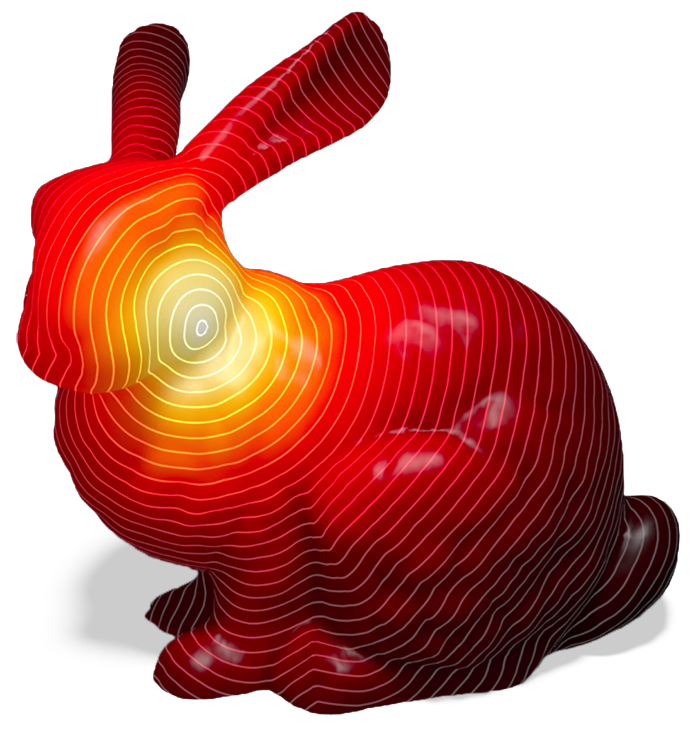
\includegraphics[width=.7\textheight]{Figures/heat_bunny.png}
    \end{figure}
\end{frame}

\begin{frame}{Motivation}
    Developability
    \begin{figure}
        \centering
        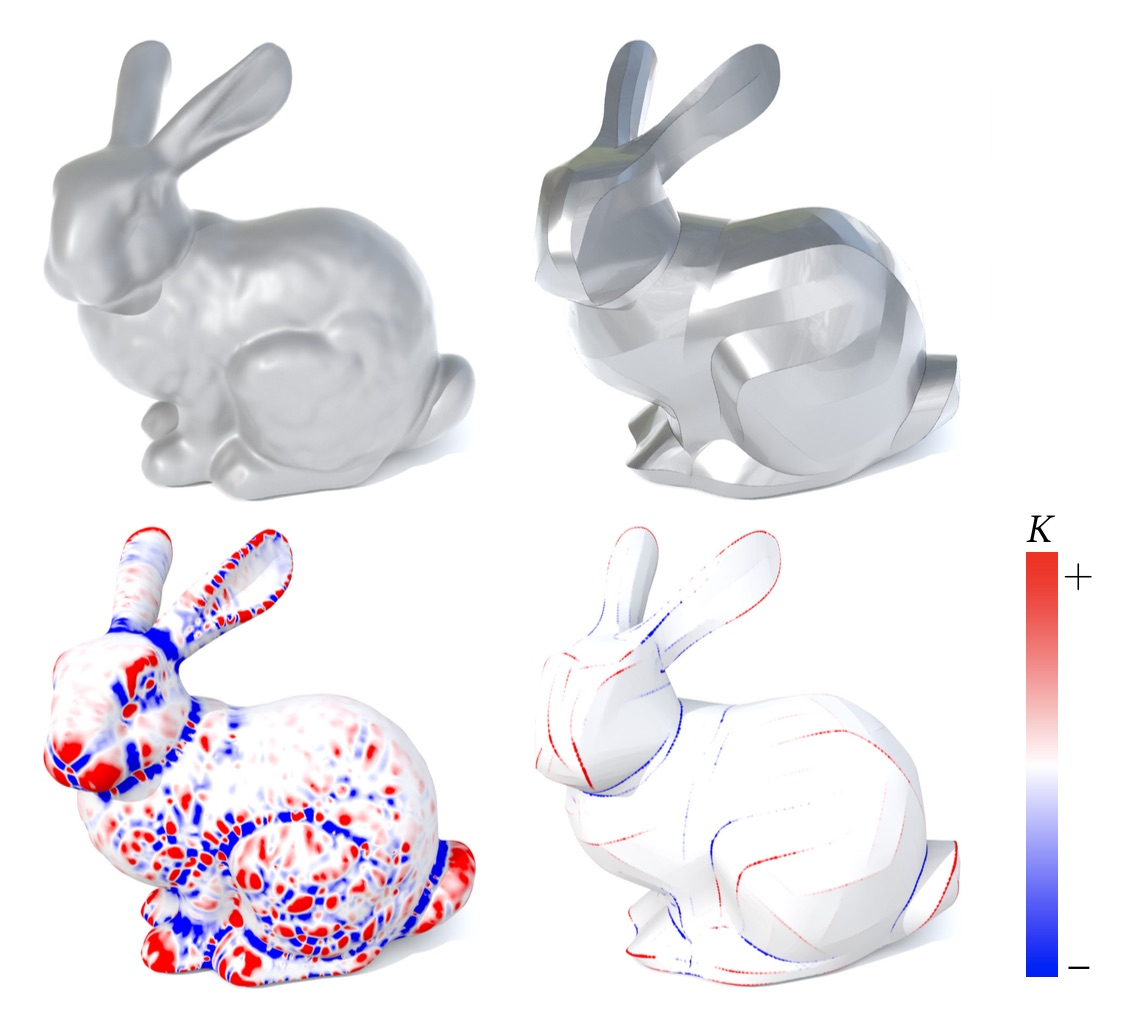
\includegraphics[width=.8\textheight]{Figures/developability_bunny.jpg}
    \end{figure}
\end{frame}

\begin{frame}{Motivation}
    Texture mapping
    \vfill
    \begin{figure}
        \centering
        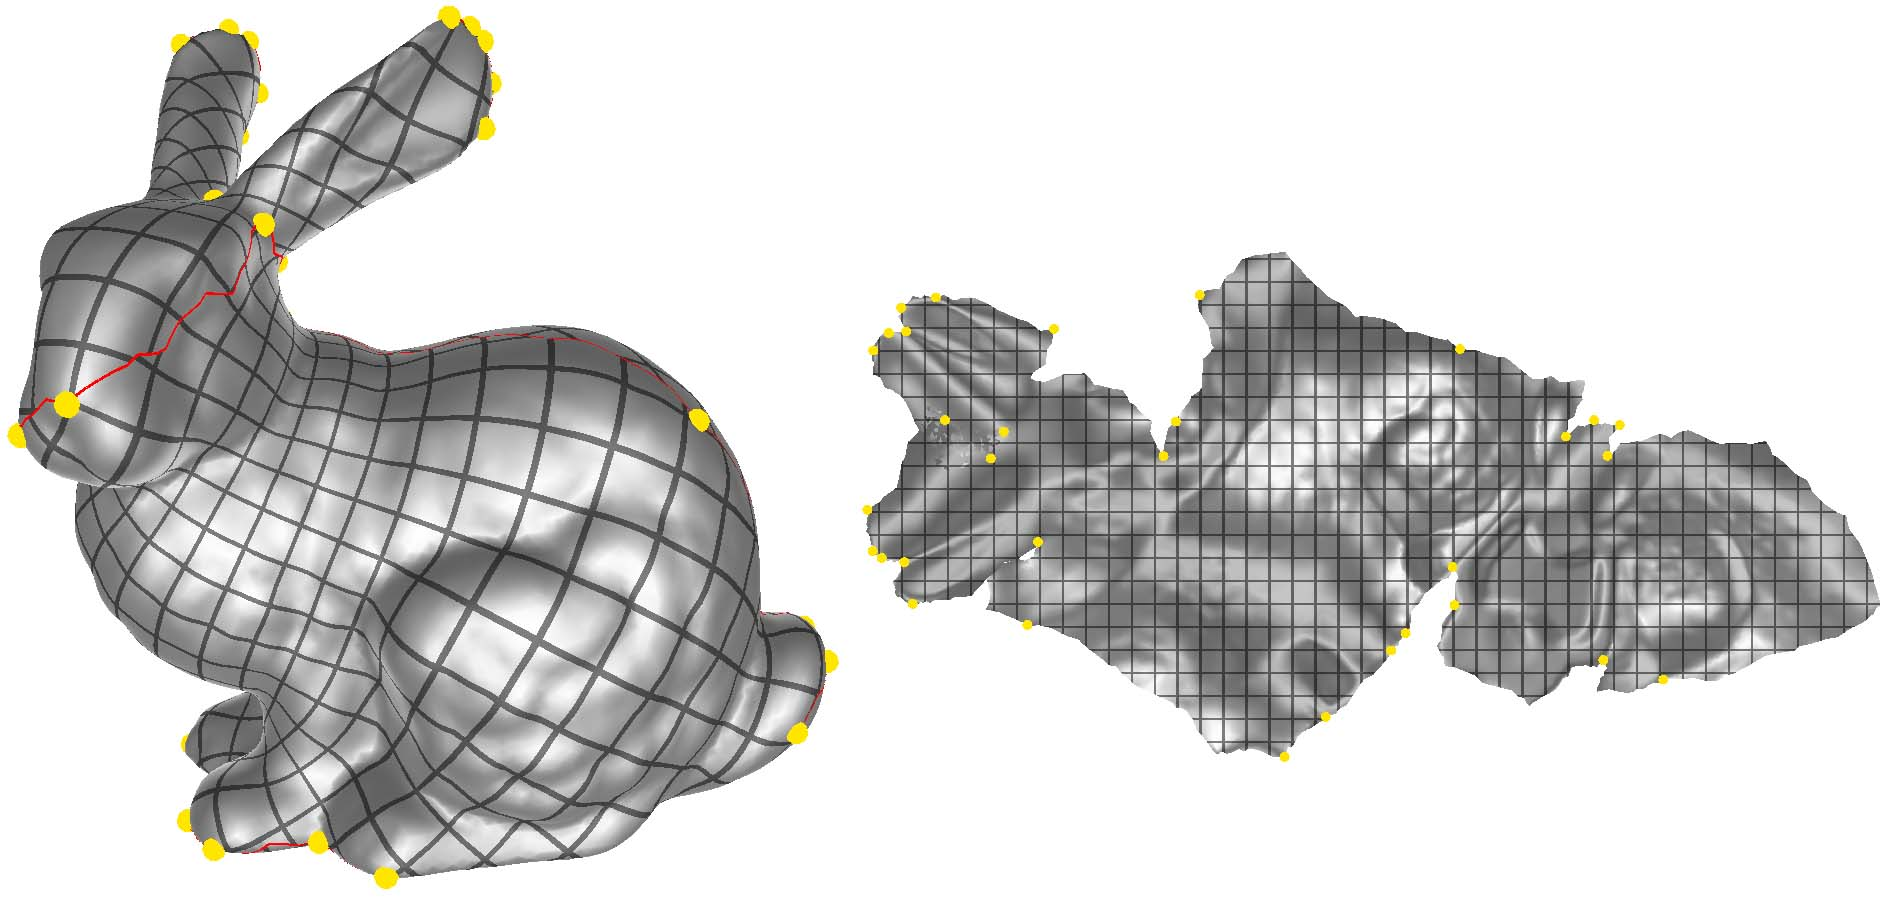
\includegraphics[width=.8\textwidth]{Figures/texture_map_bunny.jpg}
    \end{figure}
\end{frame}

\begin{frame}{Motivation}
    Direction fields
    \vfill
    \begin{figure}
        \centering
        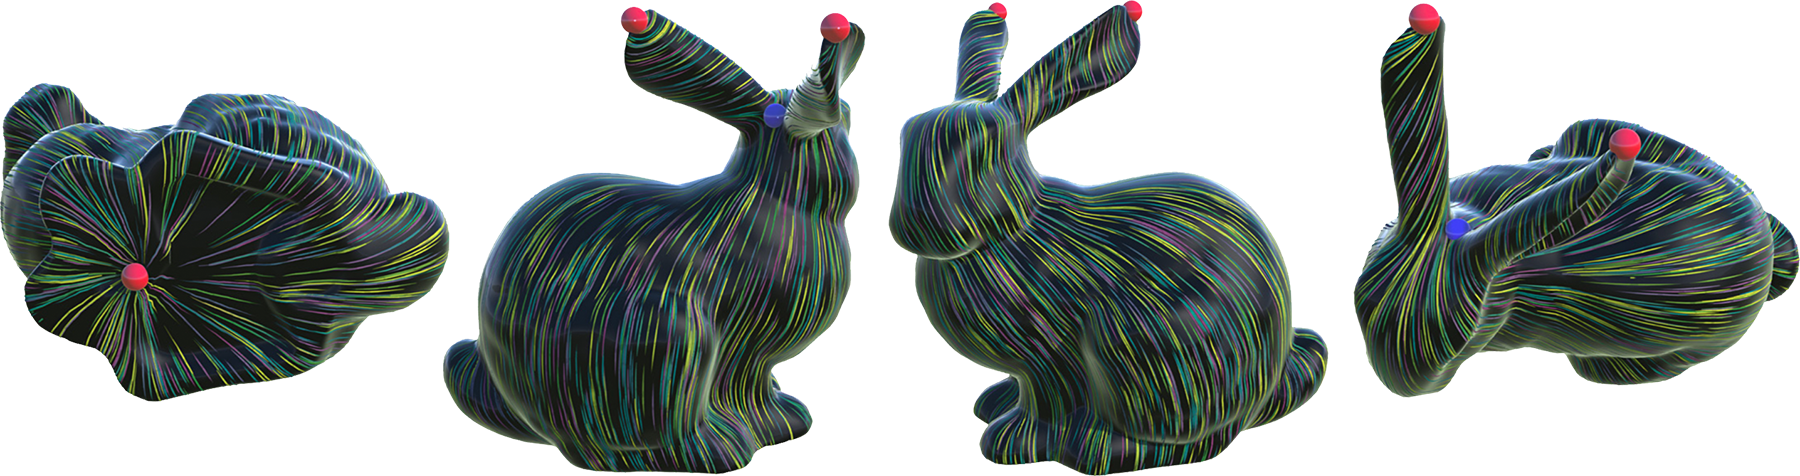
\includegraphics[width=.9\textwidth]{Figures/optimal_lines_bunny.png}
    \end{figure}
\end{frame}

\begin{frame}{Motivation}
    Geometric flow
    \vfill
    \begin{figure}
        \centering
        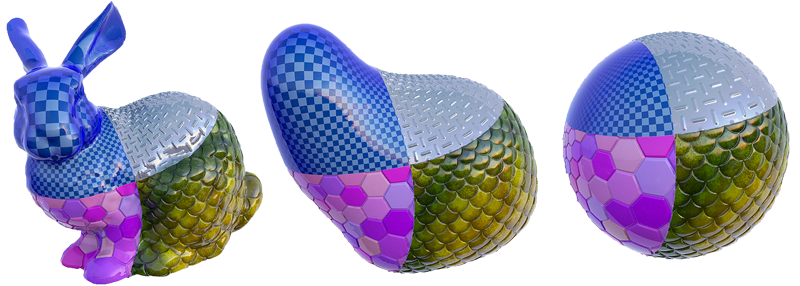
\includegraphics[width=.9\textwidth]{Figures/bunny_flow.png}
    \end{figure}
\end{frame}

\begin{frame}{Background}
    Geometric information:
    \begin{itemize}
        \item Topology.
        \item Manifold distance.
        \item Geodesics.
        \item Curvature.
    \end{itemize}
\end{frame}

\begin{frame}{What We Want}
We are given a set of points, a subdivision surface, voxel grid, spline surface, point cloud, tetrahedral mesh, or a regular grid.
\vspace*{.25cm}
    \begin{itemize}
        \item Capture geometric information.
        \item Easy to compute.
        \item Discrete theory limits to smooth theory.
    \end{itemize}
    \vspace*{.25cm}
    \begin{figure}
        \centering
        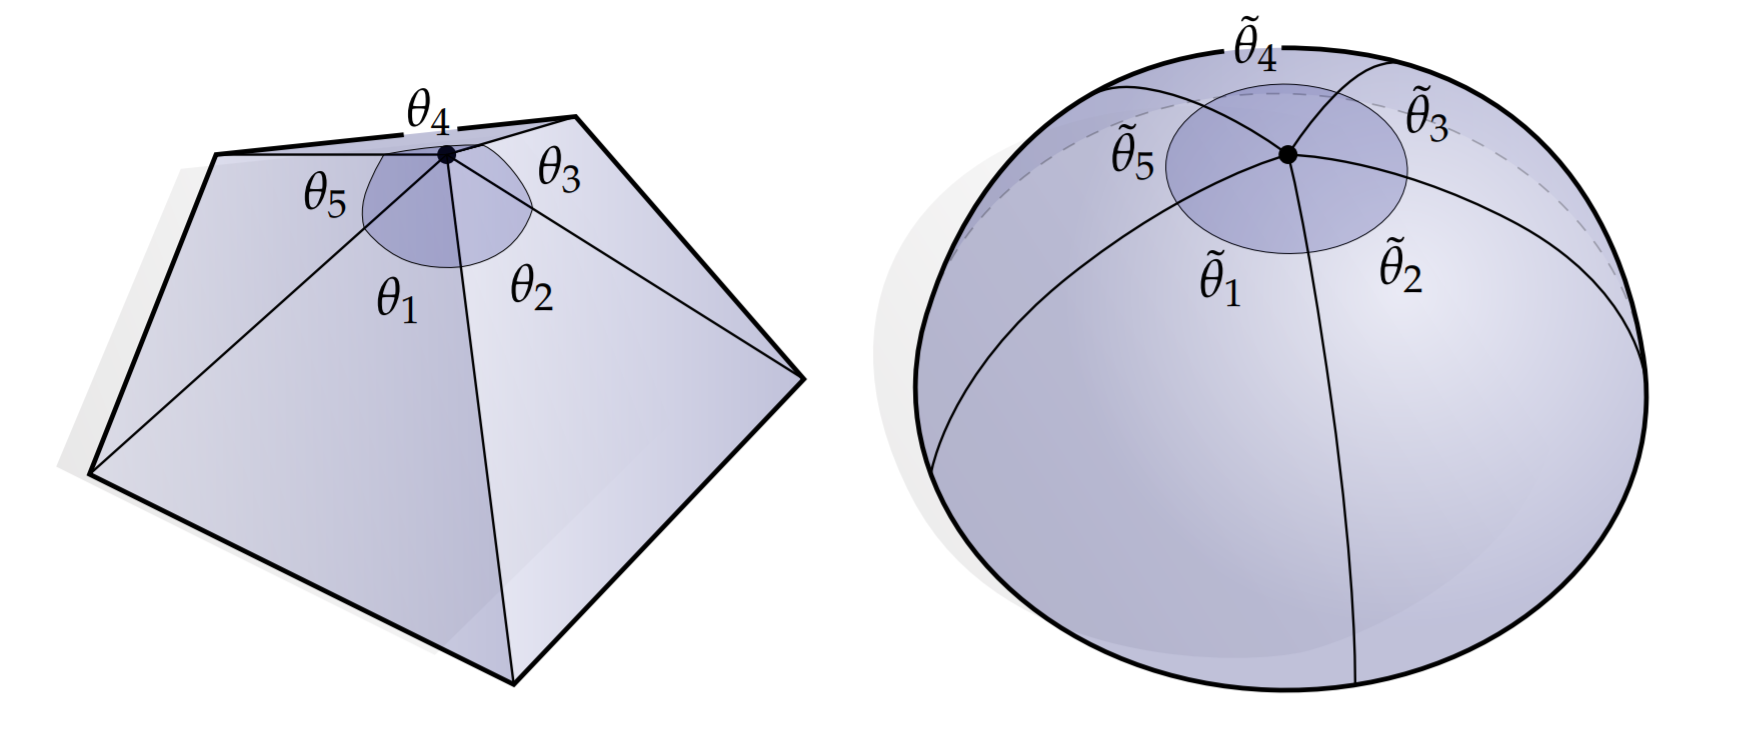
\includegraphics[width=.6\textwidth]{Figures/discrete_smooth.png}
    \end{figure}
\end{frame}

\section{Geometry}

\begin{frame}{Geometry}
    We understand the geometry of a manifold through maps $f\colon M \to \R^3$.
    \vspace*{1cm}
    \begin{figure}
        \centering
        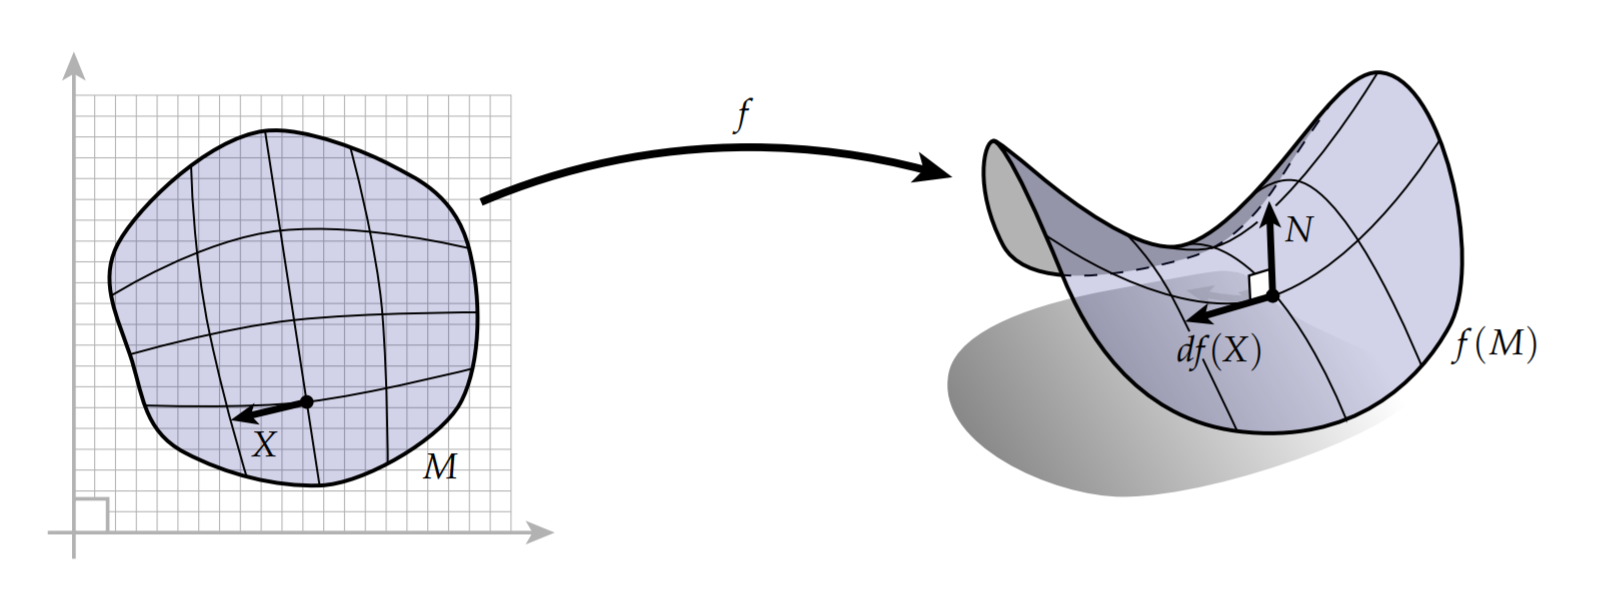
\includegraphics[width=\textwidth]{Figures/geometry_1.png}
    \end{figure}
\end{frame}

\begin{frame}{Geometry}
    We can see how areas are distorted by differentials $df$.
    \vspace*{1cm}
    \begin{figure}
        \centering
        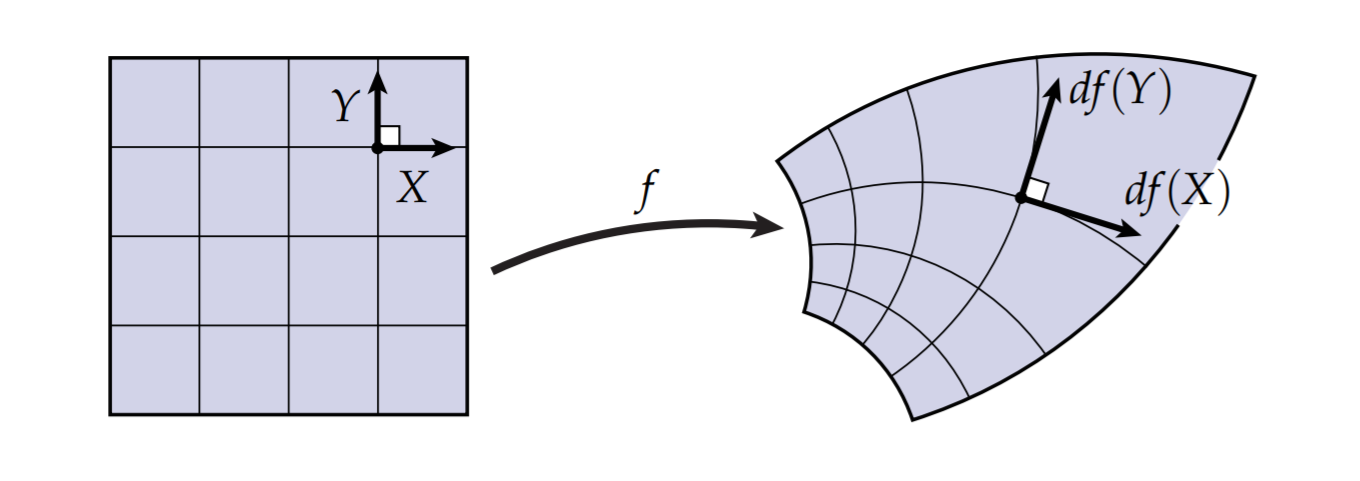
\includegraphics[width=.8\textwidth]{Figures/geometry_differentials.png}
    \end{figure}
\end{frame}

\begin{frame}{Geometry}
    Curvature in direction $X$ is captured by the changing normal $N$,
    \[
        \kappa(X)=\frac{df(X)\cdot dN(x)}{|df(X)|^2}.
    \]
        \vspace*{.25cm}
    \begin{figure}
        \centering
        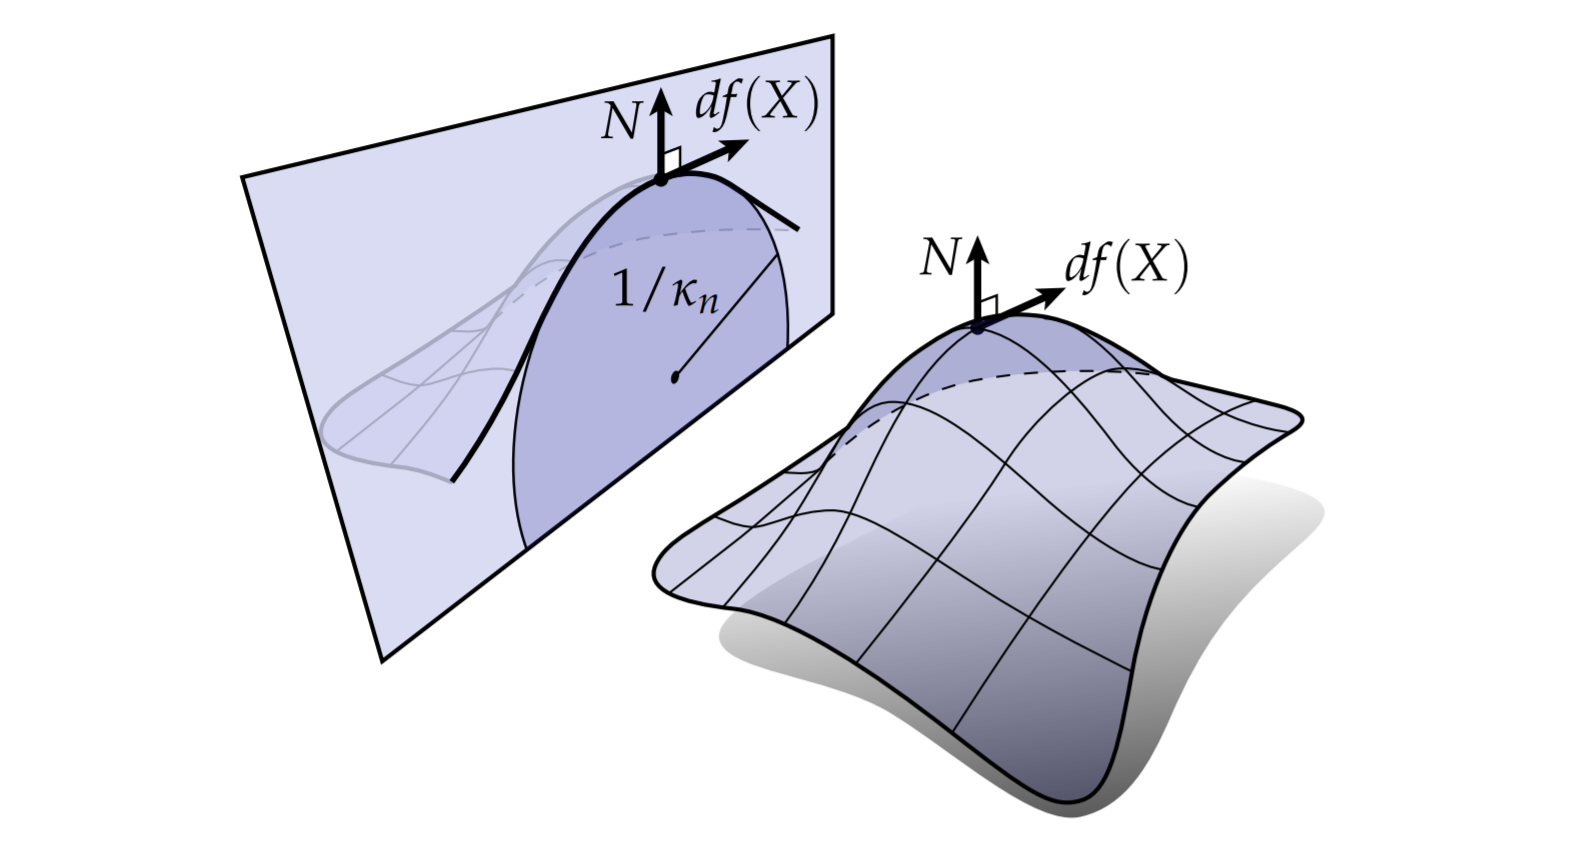
\includegraphics[width=.7\textwidth]{Figures/geometry_curvature.png}
    \end{figure}
\end{frame}

\section{Discretization}

\begin{frame}{Discretization}
    Discretization is given by coordinates.
    \vfill
    \begin{figure}
        \centering
        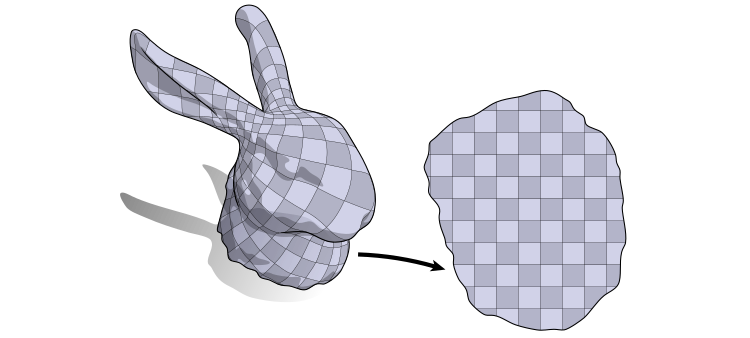
\includegraphics[width=.9\textwidth]{Figures/bunny_map.png}
    \end{figure}
\end{frame}

\begin{frame}{Discretization}
    We store the collection as a simplicial complex.
    \vspace*{1.5cm}
    \begin{figure}
        \centering
        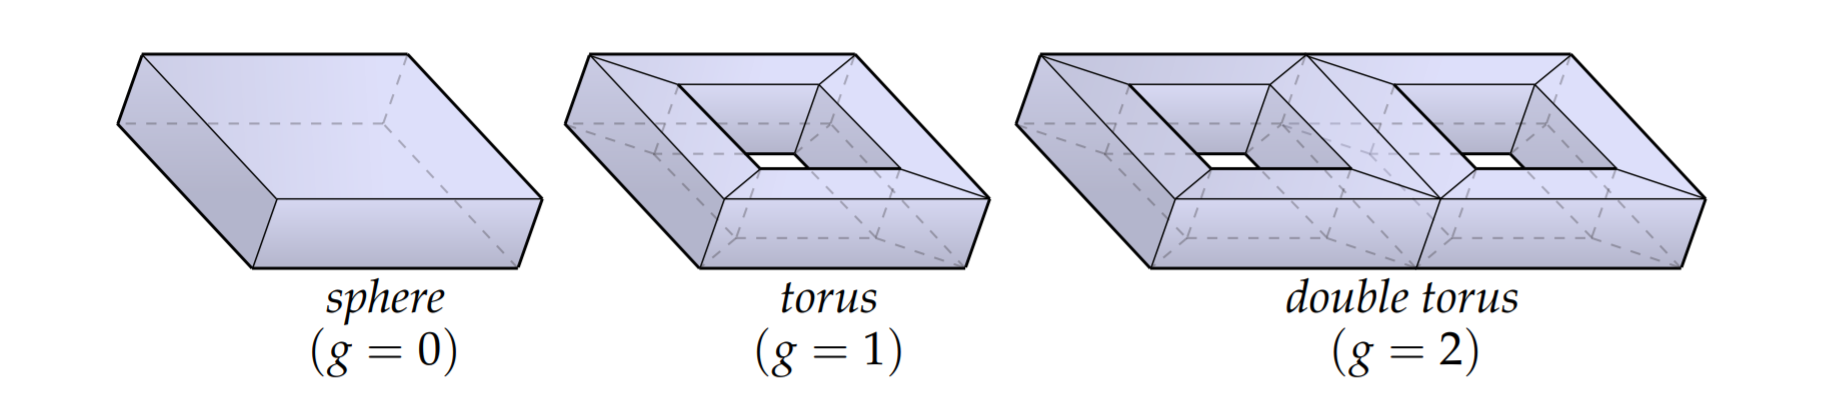
\includegraphics[width=.9\textwidth]{Figures/topological_surfaces.png}
    \end{figure}
\end{frame}

\begin{frame}{Discretization}
We interpolate between points using adjacency matrices.

\vspace*{.5cm}
Adjacency matrix $A_k$: stores face connectivity data
\begin{itemize}
    \item $k$-simplicies as columns.
    \item $k+1$-simplicies as rows.
    \item 1 in row $r$ column $c$ if $r^\mathrm{th}$ face contains the $c^\mathrm{th}$ edge. 0 otherwise.
\end{itemize}
\begin{figure}
    \centering
    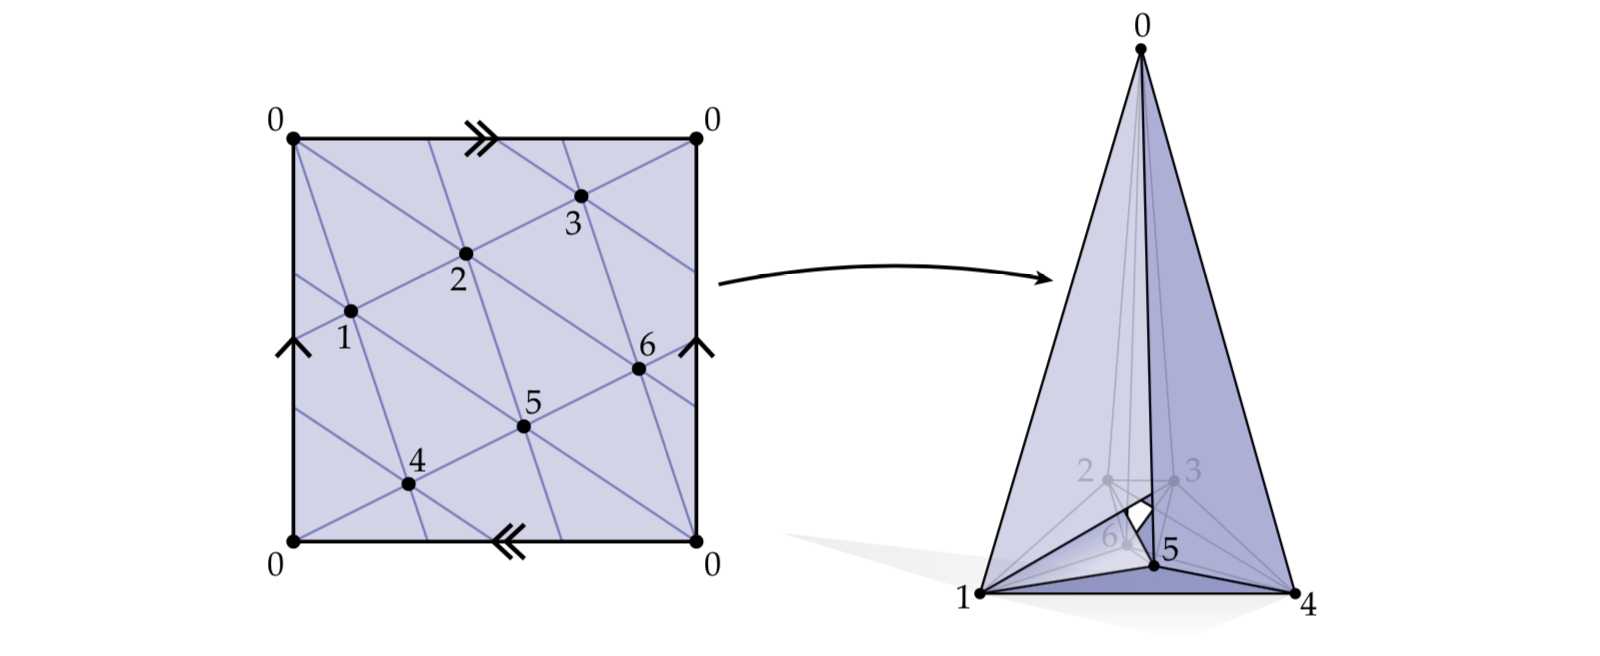
\includegraphics[width=.7\textwidth]{Figures/simplicial_complex.png}
\end{figure}
\end{frame}


\begin{frame}{Discretization}
\begin{columns}
    \begin{column}{0.48\textwidth}
        \begin{align*}
            A_0 &=\bordermatrix[{[]}]{%
            & 0 & 1 & 2 & 3 \cr
          0 & 1 & 1 & 0 & 0 \cr
          1 & 1 & 0 & 1 & 0 \cr
          2 & 1 & 0 & 0 & 1 \cr
          3 & 0 & 1 & 1 & 0 \cr
          4 & 0 & 1 & 0 & 1 \cr
          5 & 0 & 0 & 1 & 1 \cr
          }
        \end{align*}
    \end{column}
    \begin{column}{0.48\textwidth}
        \begin{figure}
            \centering
            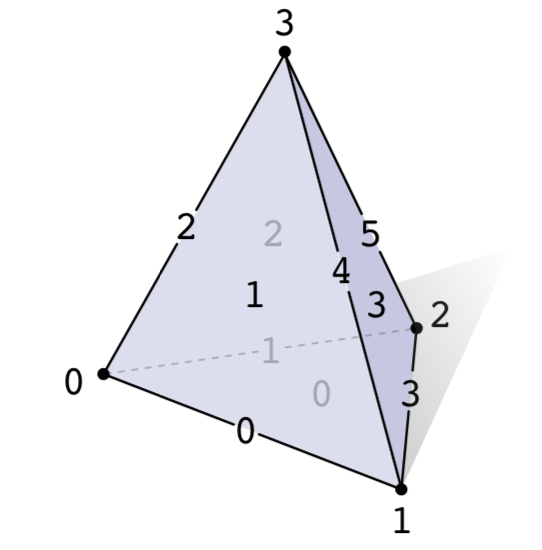
\includegraphics[width=\textwidth]{Figures/tet_surface.png}
            % \caption{Caption}
            % \label{fig:my_label}
\end{figure}
    \end{column}
\end{columns}
\end{frame}

\begin{frame}{Discretization}
\begin{columns}
    \begin{column}{0.48\textwidth}
        \begin{align*}
            A_1 &=\bordermatrix[{[]}]{%
            & 0 & 1 & 2 & 3 & 4 & 5 \cr
          0 & 1 & 1 & 0 & 1 & 0 & 0 \cr
          1 & 1 & 0 & 1 & 0 & 1 & 0 \cr
          2 & 0 & 1 & 1 & 0 & 0 & 1 \cr
          3 & 0 & 0 & 0 & 1 & 1 & 1
          }
        \end{align*}
    \end{column}
    \begin{column}{0.48\textwidth}
        \begin{figure}
            \centering
            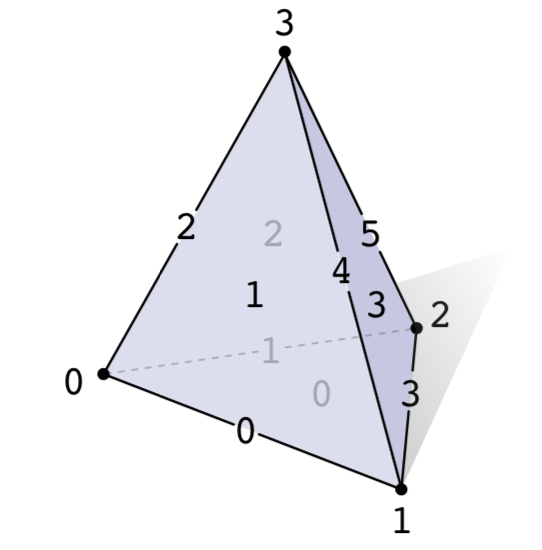
\includegraphics[width=\textwidth]{Figures/tet_surface.png}
            % \caption{Caption}
            % \label{fig:my_label}
\end{figure}
    \end{column}
\end{columns}
\pause
These are sparse!
\end{frame}

\begin{frame}{Discretization}
    Curvature is at vertices, but what is the normal?
    \vspace*{.5cm}
    \begin{figure}
        \centering
        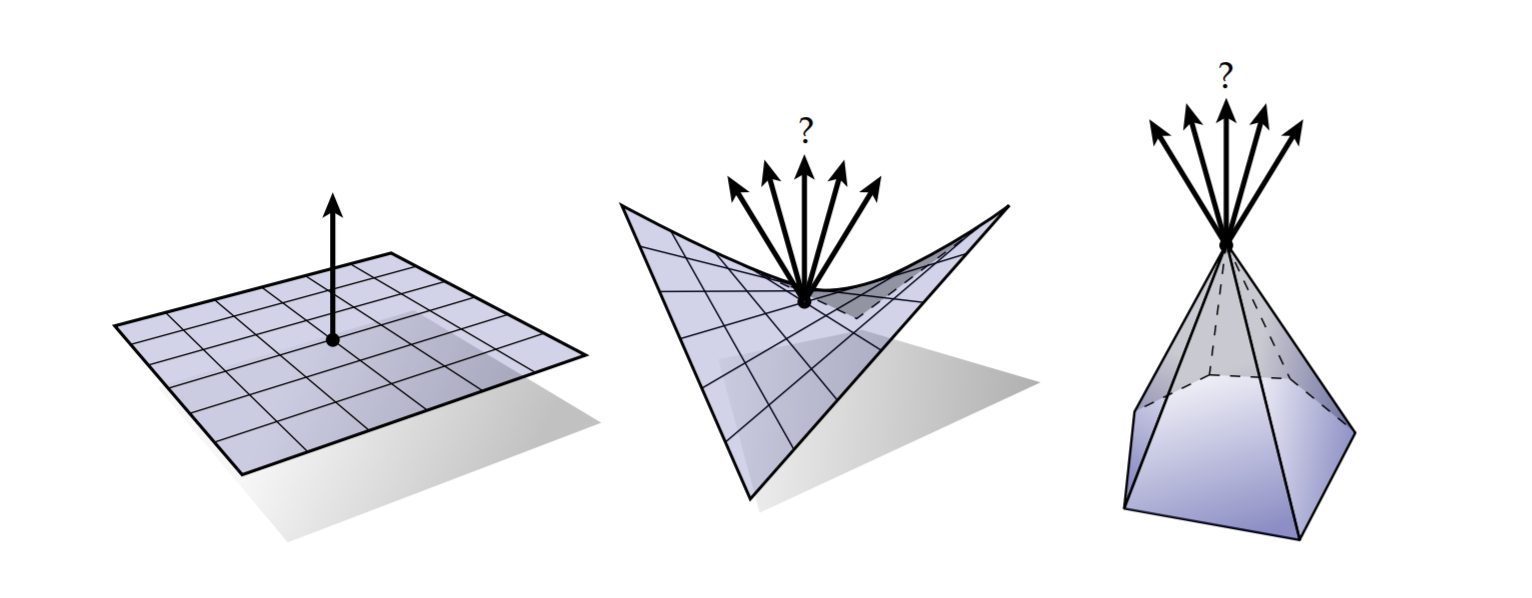
\includegraphics[width=\textwidth]{Figures/discrete_normal.png}
    \end{figure}
\end{frame}

\begin{frame}{Discretization}
    Use the normals surrounding the vertex.
    \vspace*{1cm}
    \begin{figure}
        \centering
        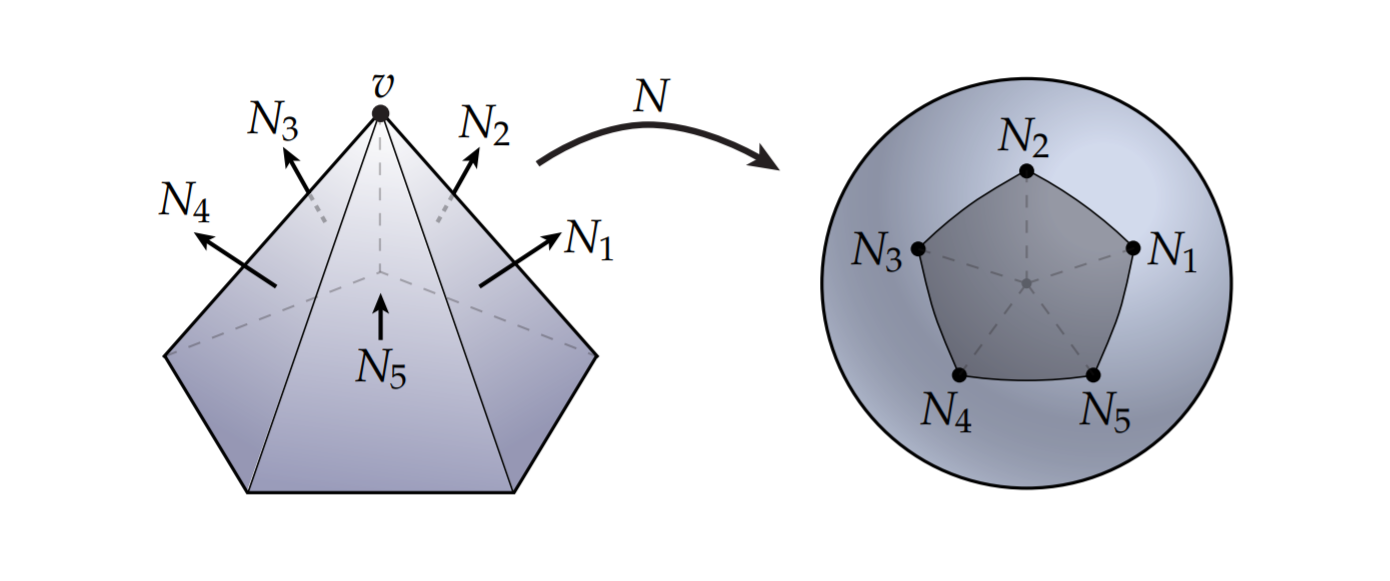
\includegraphics[width=.8\textwidth]{Figures/discrete_curvature.png}
    \end{figure}
\end{frame}

\begin{frame}{Discretization}
    Can construct the Laplacian $\Delta=\star d \star d$ by
    \begin{itemize}
        \item Let $u_i$ be the value of $u(x)$ on vertex $i$.
        \item The differential is $\nabla u \equiv (du)_{ij}=u_j-u_i$.
        \item Create the dual mesh.
        \item The Hodge dual $\displaystyle{(\star du)_{ij}=\frac{|e_{ij}^\star|}{|e_{ij}|}}(u_j-u_i)$.
    \end{itemize}
    \begin{figure}
        \centering
        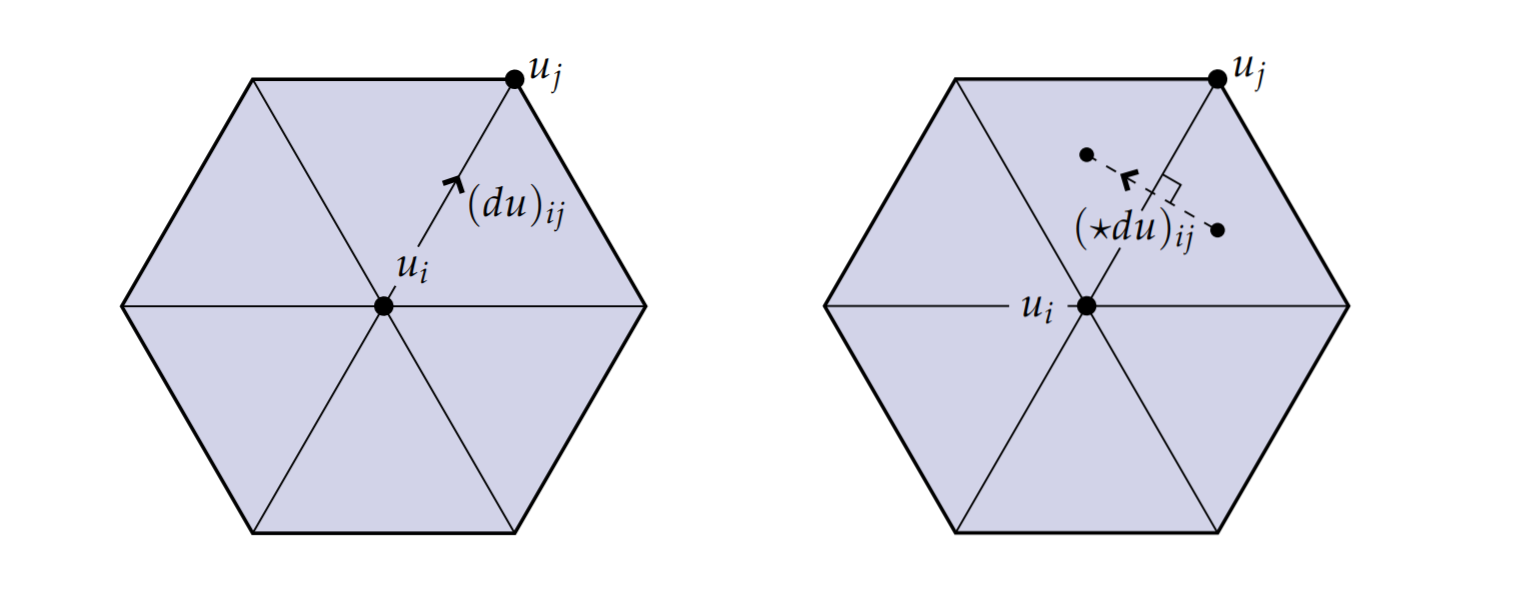
\includegraphics[width=.8\textwidth]{Figures/discrete_differentials.png}
    \end{figure}
\end{frame}

\begin{frame}{Discretization}
    The dual mesh.
    \begin{figure}
        \centering
        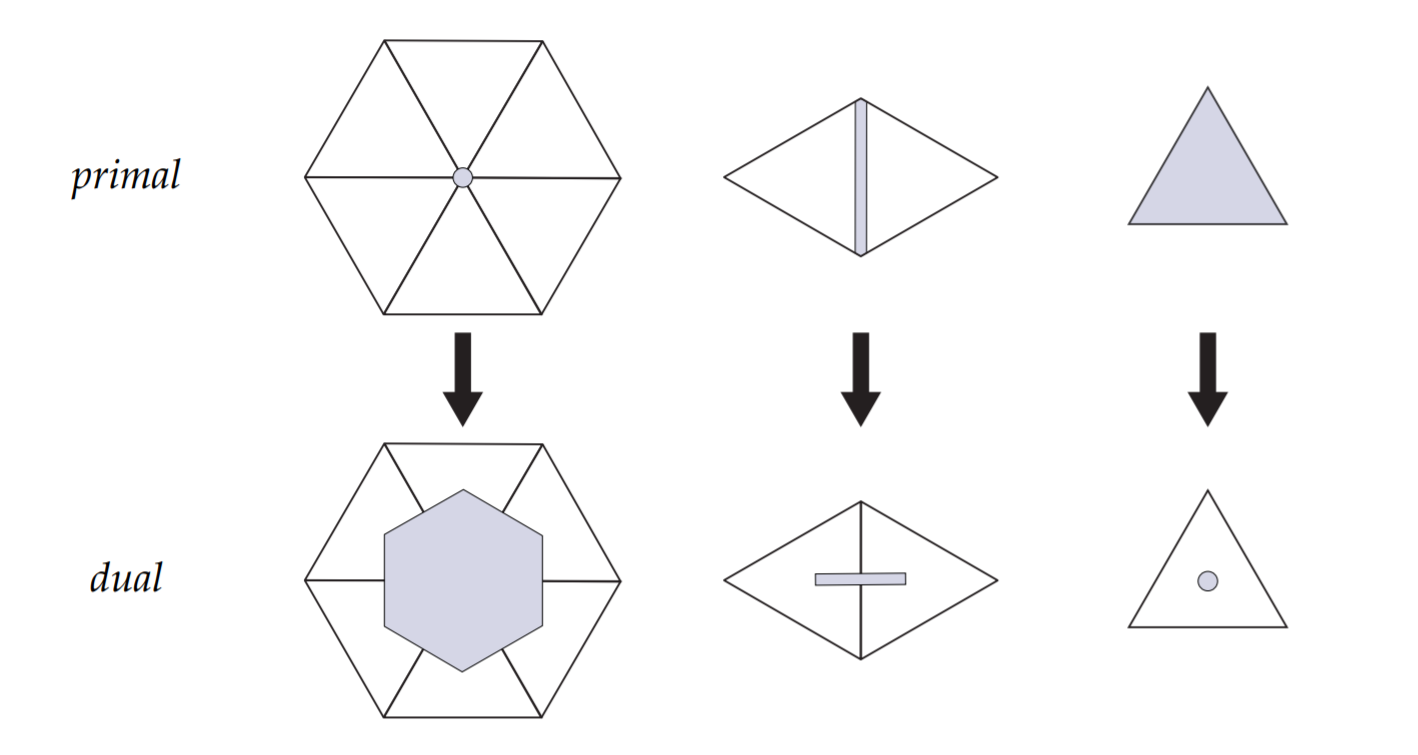
\includegraphics[width=\textwidth]{Figures/dual_mesh.png}
    \end{figure}
\end{frame}

\section{Applications}

\begin{frame}{Applications}
    Optimal direction fields.
    \begin{itemize}
        \item Goal:
        \[
        \underbrace{\min_u \int |\nabla u|^2}_{\textrm{Dirchlet energy}}.
        \]
        \item Reformulate to let $u$ be unit length (which requires energy to be modified)
        \[
        \min_{|\tilde{u}|=1}\left(\underbrace{\min_{\|a\|=1}}_{\textrm{Rescaling}}\int_M |\nabla (a \tilde{u})|^2dA\right) ~\iff~ \underbrace{\Delta u = \lambda u}_{\textrm{Smallest Eigenvalue Problem}}.
        \]
    \end{itemize}
\end{frame}

\begin{frame}{Applications}
    Discretizing the problem.
    \begin{itemize}
        \item Let $\Psi_i$ be basis tangent vector at a vertex.
        \item We can define the mass matrix $M_{ij}=\langle\langle \Psi_i,\Psi_j\rangle\rangle$.
        \item Then the stiffness matrix $A_{ij}=\langle\langle \nabla \Psi_i, \nabla \Psi_j\rangle \rangle$.
        \item Then the discretization is
        \[
        \Delta u = \lambda u ~\iff~ Au=\lambda Mu.
        \]
    \end{itemize}
\end{frame}

\begin{frame}{Applications}
    Generating a texture from optimal direction fields.
    \begin{figure}
        \centering
        \includegraphics[width=.8\textwidth]{Figures/CornMan.png}
    \end{figure}
\end{frame}

\begin{frame}{Applications}
    Computing manifold distance via the heat method.
    \begin{itemize}
        \item Start with Eikonal equation: $|\nabla \phi|=1$.
        \item Use Varadhan's formula: $\phi = \lim_{t\to 0} \sqrt{-4t\log k_t}$.
        \item Want a vector field $X\approx \nabla \phi$, so we solve
        \[
        \min_{\phi} \|\nabla \phi -X \|^2 ~\iff~ \underbrace{\Delta \phi = \nabla \cdot X}_{\textrm{Linear!}}.
        \]
        \item Discretize using the discrete differential.
    \end{itemize}
\end{frame}

\begin{frame}{Applications}
    Organisms with interesting growth.
    \begin{figure}
        \centering
        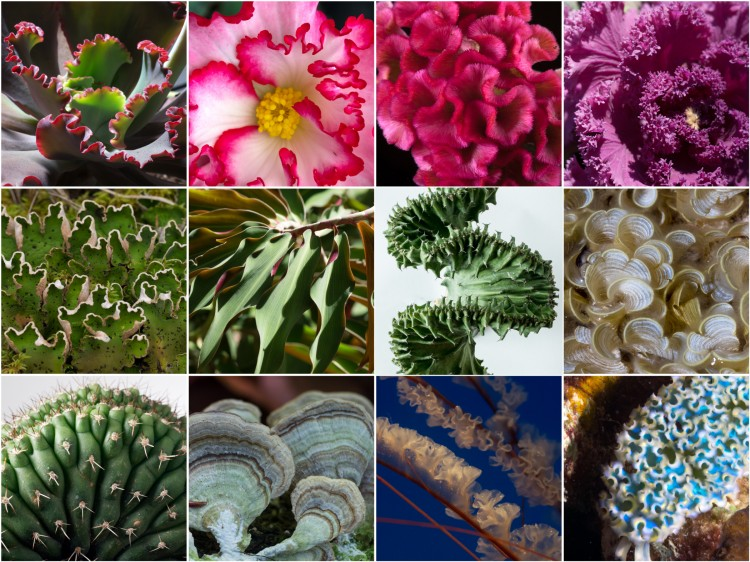
\includegraphics[width=.8\textwidth]{Figures/ruffledStuff-750x562.jpg}
    \end{figure}
\end{frame}

\begin{frame}{Floraform}
    \animategraphics[loop,controls,width=\linewidth]{20}{wireframeadapt/wireframeAdapt-}{0}{19}
\end{frame}

\section{Conclusions}

\begin{frame}{Conclusions}
    \begin{itemize}
        \item A different methodology for constructing smooth information from a discrete setting.
        \item Works on many types of data types.
        \item Generating textures is automated and can be further refined.
        \item Allows for quick computation of certain information.
        \begin{itemize}
            \item Heat method is 20 times faster than fast marching.
        \end{itemize}
        \item Texture mapping is automated and conformal structure guarantees less distortion.
        \item Can improve mesh quality and smooth meshes.
    \end{itemize}
\end{frame}


\begin{frame}{References}
    \begin{itemize}
        \item \emph{Discrete Differential Geometry: An Applied Introduction} by Keenan Crane.
        \item Lectures by Peter Schroeder and Keenan Crane.
    \end{itemize}
    
\end{frame}
\end{document}